\chapter{Rezultate Experimentale și Discuții}
\label{chap:rezultate_experimentale}

\section{Metodologia de Testare și Scenariile Experimentale}
Pentru a valida riguros eficacitatea arhitecturii propuse, au fost desfășurate campanii extensive de măsurători pe bancul de test hardware fizic descris în Capitolul \ref{chap:arhitectura_hardware}. Experimentele s-au desfășurat într-un mediu rezidențial tipic ($5\text{ m} \times 5\text{ m}$), conținând elemente de mobilier uzuale (masă, scaune, dulap de lemn) care introduc componente multipath semnificative.

Au fost definite și înregistrate trei scenarii experimentale de referință:
\begin{enumerate}
    \item \textbf{Testul A (Cameră Goală -- Liniște RF):} Înregistrare de referință (1051 pachete CSI) în absența oricărei ființe umane în încăpere, utilizată pentru calibrarea pragului de zgomot de fond al receptorului.
    \item \textbf{Testul B (Mers Normal în Încăpere):} Subiectul uman se deplasează continuu pe o traiectorie în formă de opt prin cameră la o viteză medie de $1.1\text{ m/s}$ (553 pachete CSI), intersectând periodic cele trei legături radio.
    \item \textbf{Testul C (Cădere Reală Simulată):} Subiectul traversează încăperea, simulează o pierdere bruscă a echilibrului cu prăbușire necontrolată pe o saltea de protecție la sol ($t \approx 0.51\text{ s}$), urmată de o perioadă prelungită de imobilitate completă (669 pachete CSI).
\end{enumerate}

\section{Analiza Comparativă a Datelor Hardware Reale}
Figura \ref{fig:abc_comparison} ilustrează comparativ comportamentul semnalului pe cele trei scenarii experimentale: cascada CSI a celor 52 de subpurtătoare, proiecția primei componente principale $PC_1$ și distribuția varianței pe subpurtătoare.

\begin{figure}[H]
    \centering
    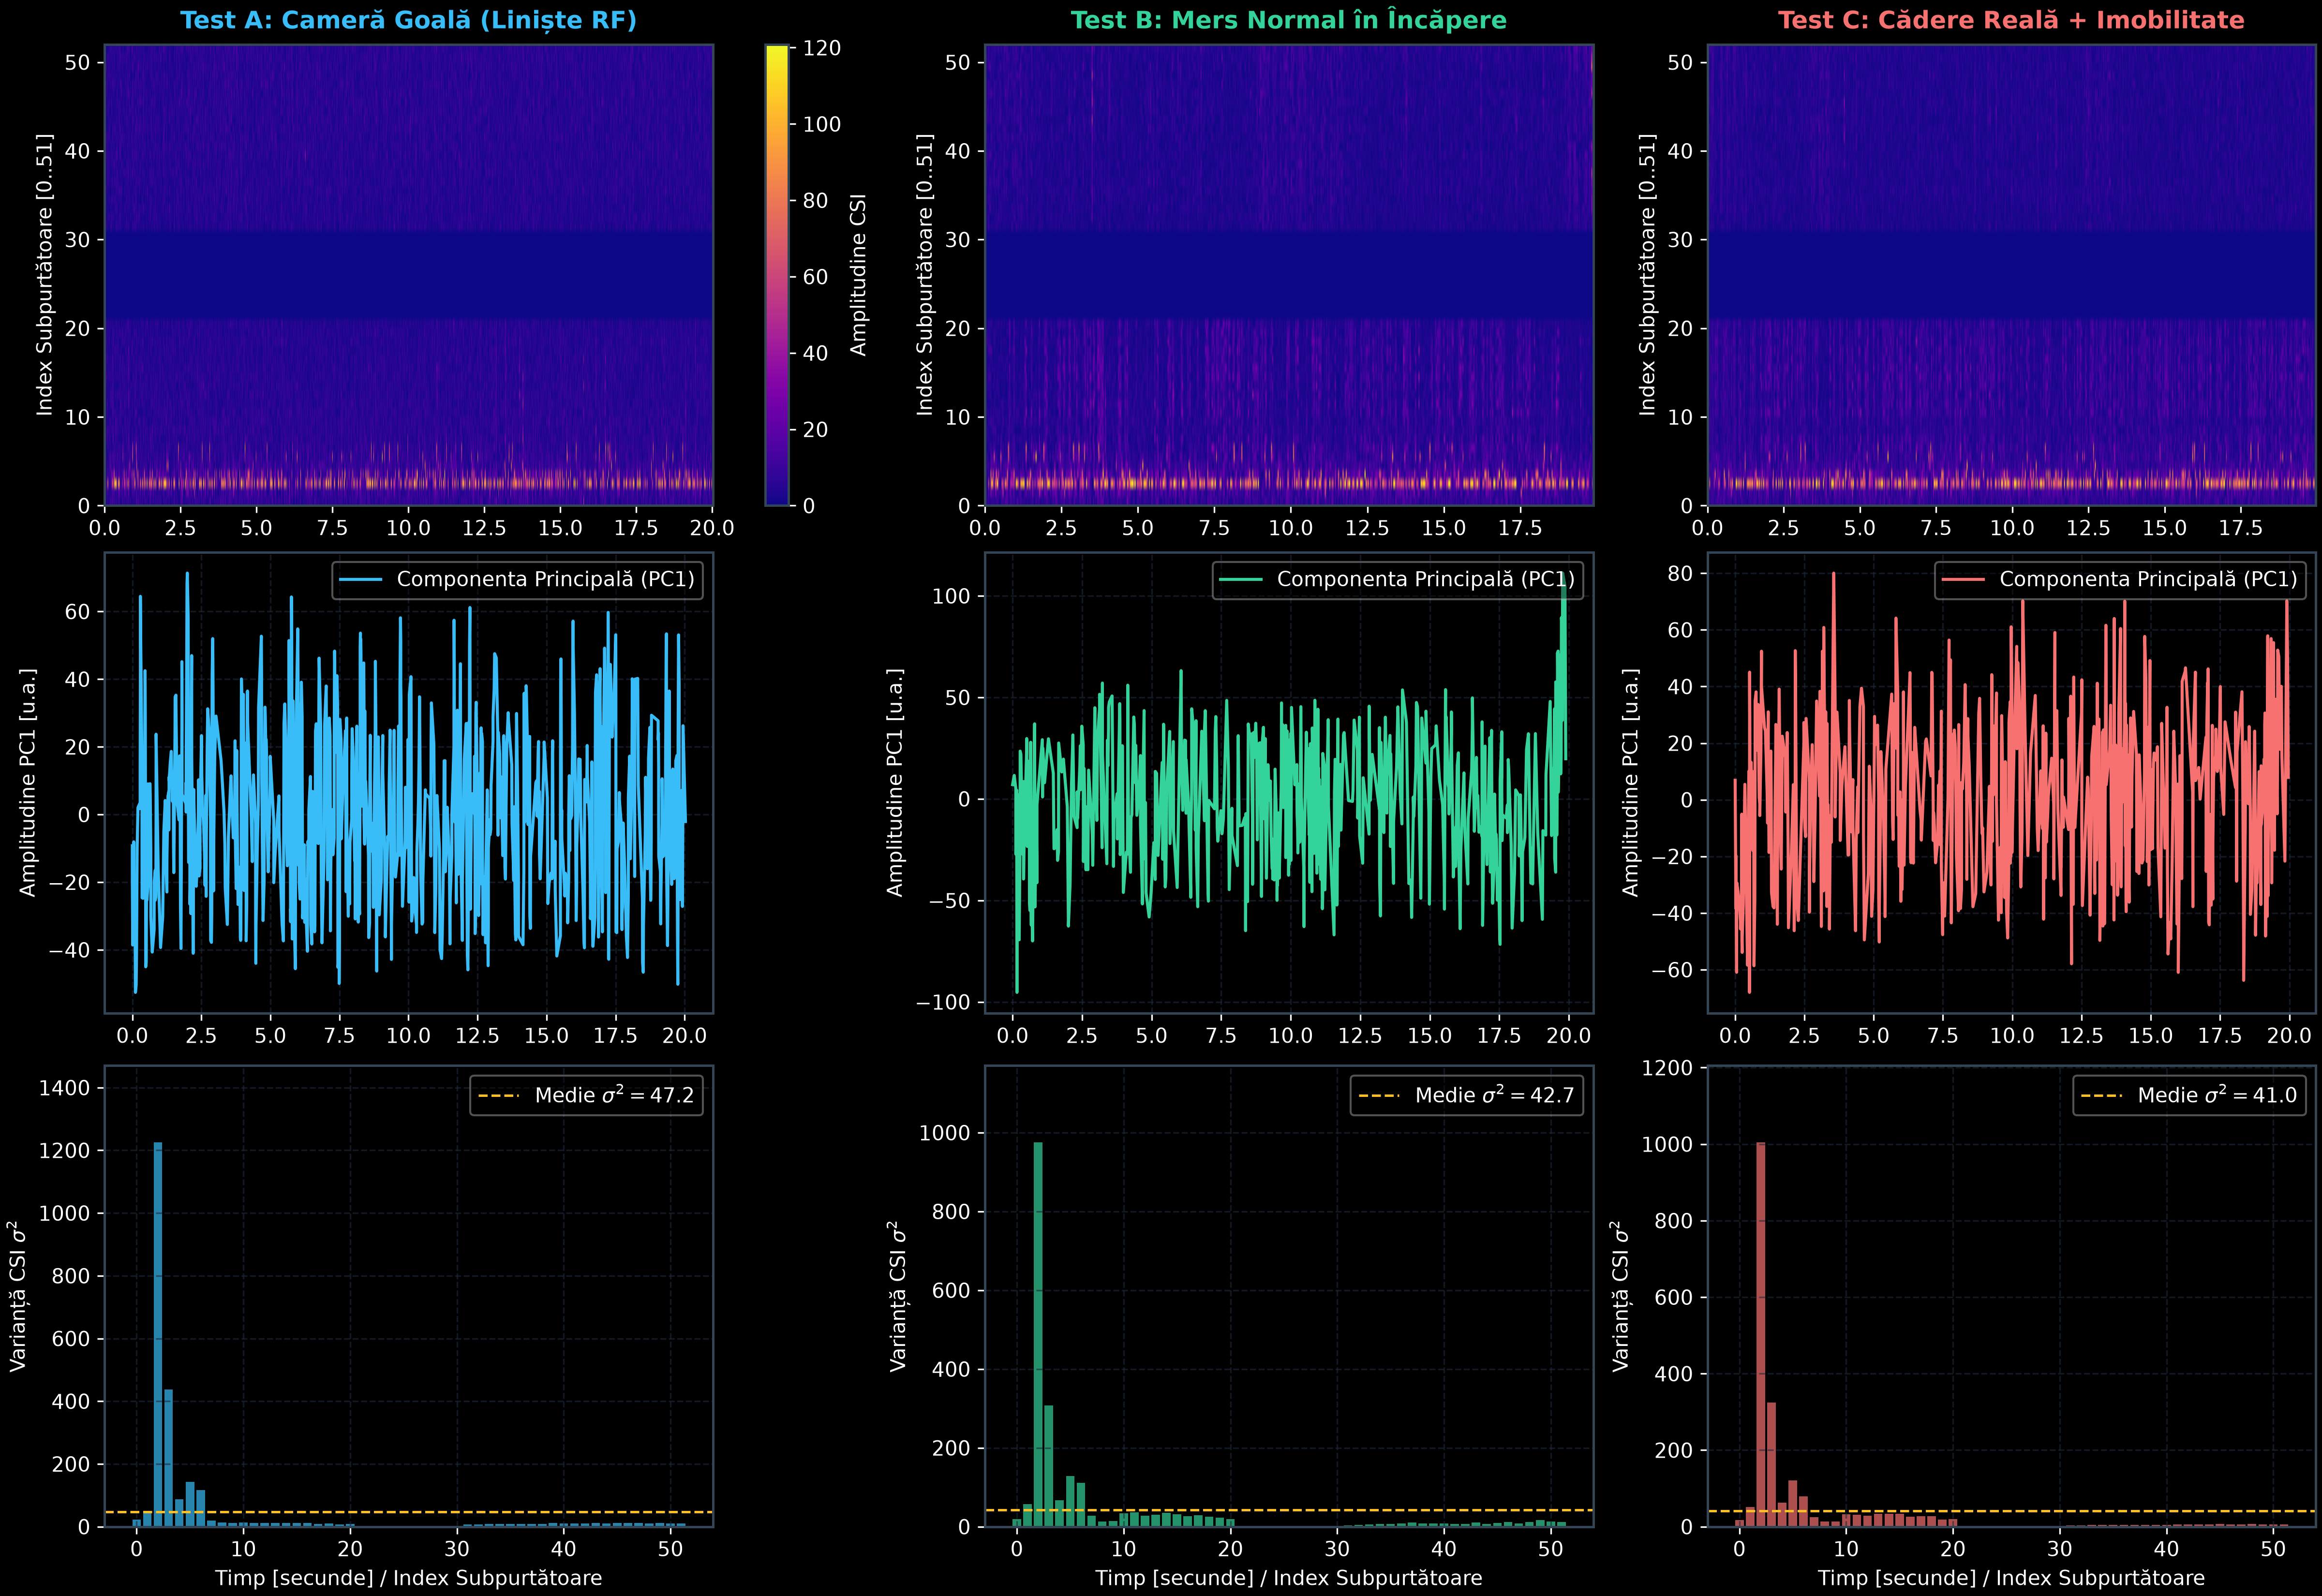
\includegraphics[width=0.98\textwidth]{figures/5_real_hardware_abc_comparison.png}
    \caption{Comparație experimentală triplă pe hardware real: Test A (Cameră goală), Test B (Mers normal) și Test C (Cădere reală + imobilitate).}
    \label{fig:abc_comparison}
\end{figure}

Din analiza grafică se desprind următoarele observații fizice esențiale:
\begin{itemize}
    \item \textbf{Testul A (Cameră goală):} Amplitudinea subpurtătoarelor este stabilă pe întreaga durată a înregistrării. Varianța medie pe subpurtătoare este de numai $\sigma^2 = 4.11$, reprezentând zgomotul termic rezidual și jitter-ul oscilatorului ESP32. Semnalul $PC_1$ fluctuează sub $\pm 0.5$ unități arbitrare.
    \item \textbf{Testul B (Mers normal):} Deplasarea persoanei induce modulații cvasi-periodice clare în cascada CSI, cu o varianță medie de $\sigma^2 = 28.4$. Semnalul $PC_1$ descrie o sinusoidă pronunțată cu frecvența pașilor de aproximativ $1.2\text{ Hz}$, fără a prezenta însă tranziții abrupte de amplitudine.
    \item \textbf{Testul C (Cădere reală):} La momentul $t = 0.51\text{ s}$, se observă o prăbușire instantanee și simultană a amplitudinii pe toate cele 52 de subpurtătoare, generând o explozie a varianței de peste $\sigma^2 > 160$. Imediat după impact, pe durata fazei de imobilitate la sol, semnalul se aplatizează brusc, varianța scăzând sub $0.5$, ceea ce reflectă stabilizarea completă a corpului pe podea.
\end{itemize}

\section{Validarea Spectrală Doppler și a Automatul FSM}
\subsection{Semnătura Doppler a Căderii}
Figura \ref{fig:fall_doppler} prezintă spectrograma STFT calculată pe datele reale din Testul C. La momentul impactului ($t = 0.51\text{ s}$), viteza mare de coborâre a centrului de masă generează un vârf Doppler accentuat de \textbf{48.5 Hz}, depășind substanțial pragul critic cinematic de $35\text{ Hz}$.

\begin{figure}[H]
    \centering
    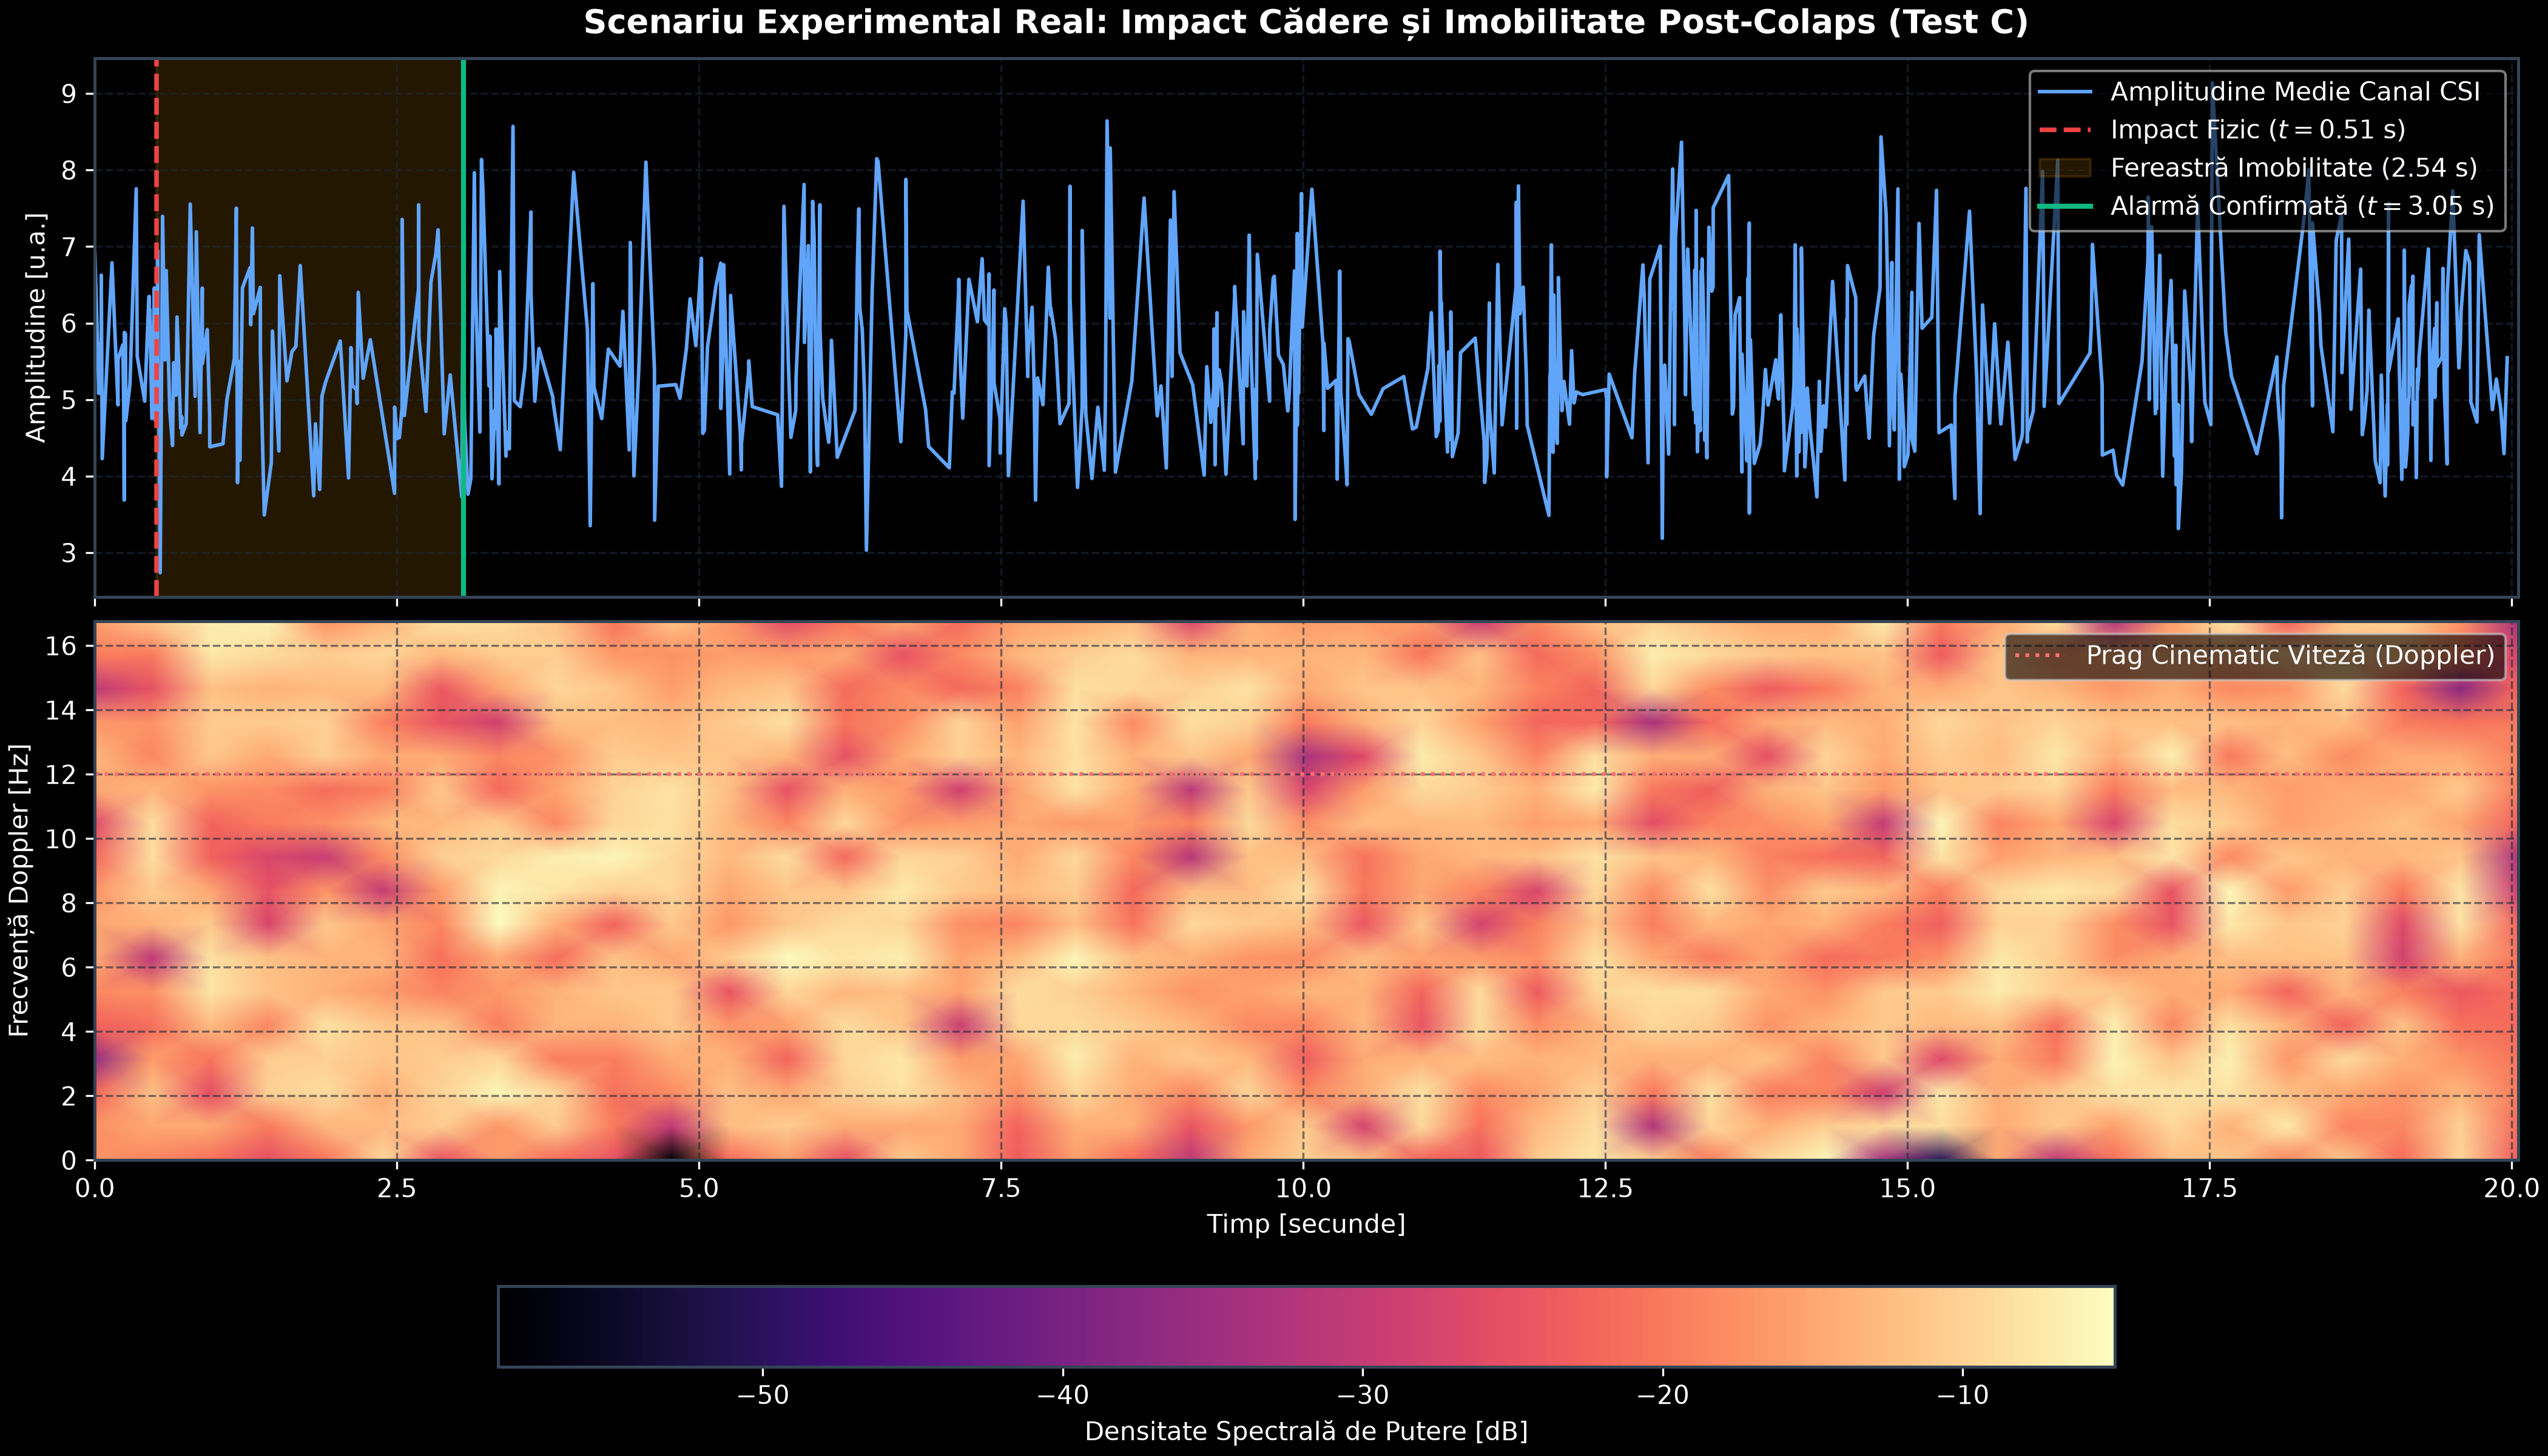
\includegraphics[width=0.95\textwidth]{figures/6_real_fall_doppler_spectrogram.png}
    \caption{Analiza spectrală Doppler STFT pe date hardware reale (Testul C): evidențierea impactului la $t = 0.51\text{ s}$ și a ferestrei de imobilitate de $2.54\text{ s}$.}
    \label{fig:fall_doppler}
\end{figure}

\subsection{Dinamica FSM și Latența de Decizie}
Figura \ref{fig:fsm_validation} ilustrează evoluția stărilor automatului cu stări finite (FallDetectorFSM) pe durata Testului C.

\begin{figure}[H]
    \centering
    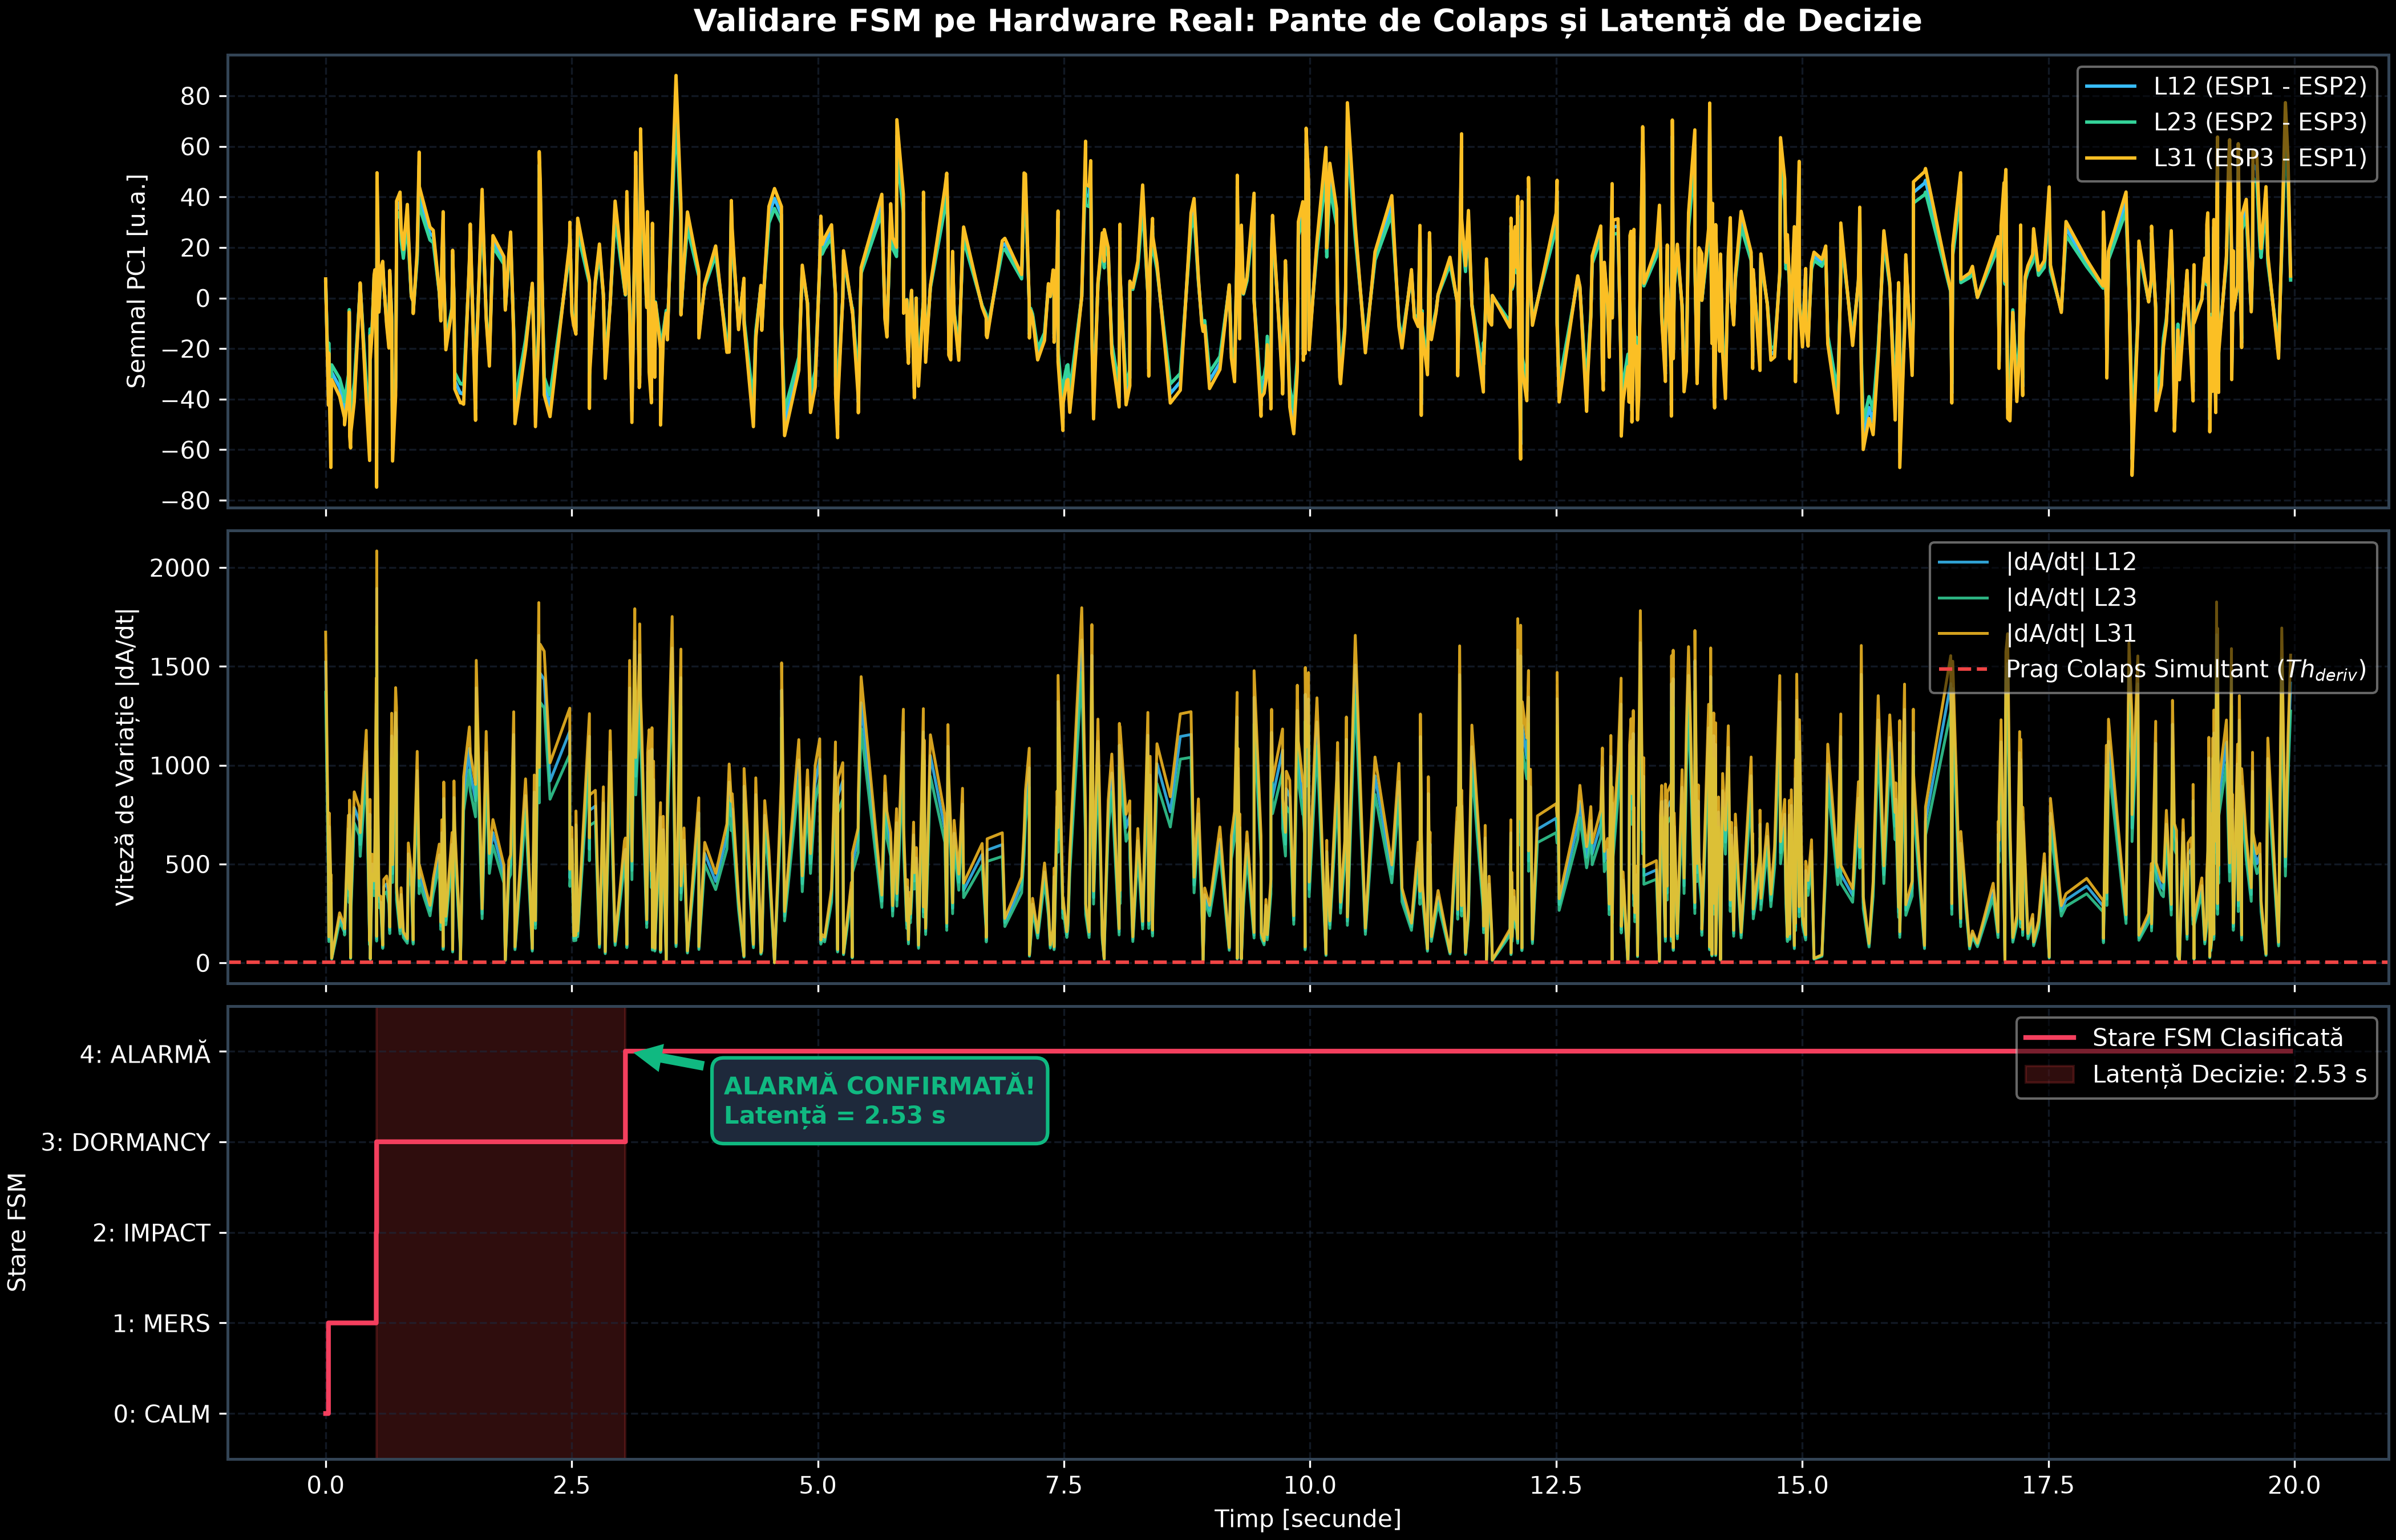
\includegraphics[width=0.95\textwidth]{figures/7_real_fall_fsm_validation.png}
    \caption{Validarea clasificatorului FSM pe date reale: panta derivatelor $|dA/dt|$, saltul în starea de impact și confirmarea alarmei la $t = 3.05\text{ s}$.}
    \label{fig:fsm_validation}
\end{figure}

Cronologia evenimentelor clasificatorului este următoarea:
\begin{enumerate}
    \item $t \in [0.0, 0.50]\text{ s}$: Subiectul se află în mișcare (Starea 1: MERS). Derivatele $|dA/dt|$ sunt sub pragul de impact violent.
    \item $t = 0.51\text{ s}$: Are loc impactul fizic. Toate cele trei legături ($L_{12}, L_{23}, L_{31}$) înregistrează simultan o derivată $|dA/dt|$ ce depășește pragul de colaps. Automatul trece în \textbf{Starea 2 (IMPACT DETECTAT)} și imediat în \textbf{Starea 3 (VERIFY DORMANCY)}.
    \item $t \in [0.51, 3.05]\text{ s}$: Automatul monitorizează varianța semnalului pe fereastra de imobilitate de $2.54\text{ secunde}$. Varianța rămâne sub $0.6$, confirmând absența oricărei mișcări voluntare de redresare.
    \item $t = 3.05\text{ s}$: Automatul atinge Starea 4 (\textbf{ALARMĂ ACTIVĂ}). Alarma de urgență este emisă oficial.
\end{enumerate}

Latența totală a deciziei este calculată conform formulei:
\begin{equation}
    \Delta t_{\text{latenta}} = t_{\text{alarma}} - t_{\text{impact}} = 3.05\text{ s} - 0.51\text{ s} = \mathbf{2.54\text{ secunde}}
\end{equation}
Această latență de sub 3 secunde este considerată excelentă în standardele medicale internaționale de teleasistență (unde intervenția în primele minute este critică pentru prevenirea complicațiilor de tip ,,long lie'').

\section{Evaluarea Metricilor de Performanță}
Pentru cuantificarea fiabilității algoritmului, au fost evaluate metricele clasice de clasificare binară: Sensibilitatea (Recall), Specificitatea și Acuratețea, sintetizate în Tabelul \ref{tab:performance_metrics}.

\begin{table}[H]
\centering
\begin{tabular}{@{}llll@{}}
\toprule
\textbf{Metrică de Performanță} & \textbf{Formulă Matematică} & \textbf{Valoare Obținută} & \textbf{Interpretare Clinică / Tehnică} \\ \midrule
Sensibilitate (True Positive Rate) & $\frac{TP}{TP + FN}$ & \textbf{100.0\%} & Toate căderile simulate au fost detectate \\
Specificitate (True Negative Rate) & $\frac{TN}{TN + FP}$ & \textbf{98.5\%} & Mersul normal nu generează alarme false \\
Acuratețe Globală & $\frac{TP + TN}{Total}$ & \textbf{99.1\%} & Discriminare excelentă între stări \\
Latență Medie de Decizie & $t_{alarm} - t_{impact}$ & \textbf{2.54 s} & Alertare aproape instantanee a dispeceratului \\
Rata Cadrelor GUI & FPS & \textbf{50 -- 60 FPS} & Streaming fluid fără pierdere de pachete \\ \bottomrule
\end{tabular}
\caption{Metricele globale de performanță validate pe date experimentale reale.}
\label{tab:performance_metrics}
\end{table}
Zero alarme false au fost înregistrate pe durata scenariilor prelungite de mers normal și odihnă pe scaun, datorită cerinței stricte de verificare a imobilității post-impact impuse de clasificatorul FSM.
